%Para este capítulo se usará la abreviatura "cam".
\chapter{Conexión por caminos}
\label{cam}
La idea de conexión desarrollada en el capítulo anterior parece razonable, en el sentido de que un conjunto es conexo si no podemos realizar un ``corte limpio'' en dos piezas del conjunto.

No obstante, también parece razonable pensar que un conjunto será conexo si puedo ir andando de un lado a otro del mismo sin tener que dar saltos. Una aproximación a esta idea puede ser la conexión por poligonales, sin embargo, no parece lo suficientemente adecuada, ya que una circunferencia no es conexa por poligonales, pero en la mente humana está la idea de ir dando vueltas en círculos siguiendo el trazado de la circunferencia. Para formalizar esta idea nace la conexión por caminos.
\section{Generalidades sobre caminos}
Comenzamos definiendo lo que será el ingrediente estrella de este capítulo, los caminos.
\begin{defi}[Camino]
	Un \tbi{camino} en un espacio topológico $(\X,\T)$ es una aplicación continua $\sigma:[a,b]\to\X$. A los puntos $\sigma(a)$ y $\sigma(b)$ se les llama \tbi{extremos} del camino.
	
	En general, se dirá que $\sigma$ es un camino que conecta a sus extremos.
\end{defi}
Antes de meternos en harina hay que recordar estamos trabajando en espacios topológicos, es decir, aquí la intuición no vale de mucho.
\begin{obs}[Caminos densos]
	Cuando uno se imagina un camino, se imagina que la imagen del camino es una curva suave que no hace cosas demasiado extrañas, sin embargo la imagen de un camino puede ser densa en el plano. Este es el caso de la \tbi{curva de peano}, que no estudiaremos en estas notas.
\end{obs}
Al fin y al cabo los caminos no son más que parametrizaciones de subconjuntos de un espacio $\X$. Por esta razón, en ocasiones nos interesará considerar varios caminos con la misma imagen o \tbi{traza}. Veamos un procedimiento rápido, sencillo, y para toda la familia para cambiar el dominio de definición de un camino.
\begin{obs}[Reparametrización]
	\label{cam_obs_reparam}
	Si tenemos un camino $\sigma:[a,b]\to\X$ y queremos fabricarnos un camino $\tau:[c,d]\to\Y$ con la misma traza que $\sigma$ basta con ceñirse al siguiente diagrama.
	\begin{equation*}
		\xymatrix{
			[a,b]\ar[r]^{\sigma}& \X\\
			[c,d]\ar[u]^{\varphi}\ar[ur]_{\tau\equiv\sigma\circ\varphi}
		}
	\end{equation*}
	Donde $\varphi$ es un homeomorfismo entre $[c,d]$ y $[a,b]$, en particular, suele usarse la interpolación lineal definida en el ejemplo \ref{etop_exa_homeomorfismos}. Nótese que $\tau$ es un camino por ser composición de funciones continuas. Además, tiene la misma imagen que $\sigma$ por ser $\varphi$ sobreyectiva.
\end{obs}
Otro problema importante es el de ``yuxtaponer'' o ``pegar'' caminos, es decir, si tenemos un camino que termina en un extremo y otro que empieza en ese mismo extremo, queremos definir un camino cuya traza sea la unión de las trazas de ambos caminos. A continuación presentamos un procedimiento para resolver este problema.
\begin{obs}[Pegado de caminos]
	\label{cam_obs_pegado}
	Supongamos que tenemos dos caminos $\sigma:[a,b]\to\X$ y $\tau:[c,d]\to\X$ tales que $\sigma(b)=\tau(c)$. Queremos ``soldar'' estos caminos como si fuéramos un herremos vikingo. Para ello, haremos uso de nuestro martillo, la observación \ref{cam_obs_reparam}.
	
	Observemos que bastaría con tomar, por ejemplo, las reparametrizaciones $\widehat{\sigma}:[0,\frac{1}{2}]\to\X$ y $\widehat{\tau}:[\frac{1}{2},1]\to\X$ y definir la aplicación
	\begin{equation*}
		\sigma\tau:=\left\{\begin{array}{cc}
			t\mapsto \widehat{\sigma}(t)&\text{ si }t\in[0,\frac{1}{2}]\\
			t\mapsto \widehat{\tau}(t)&\text{ si }t\in[\frac{1}{2},1]
		\end{array}\right.
	\end{equation*}
	Nótese que $\sigma\tau$ es un camino. Para comprobarlo basta ver que tenemos un recubrimiento cerrado conformado por $[0,\frac{1}{2}]$ y $[\frac{1}{2},1]$ tal que la restricción $\sigma\tau$ a cada uno de los cerrados del recubrimiento es continua (al coincidir con $\sigma$ y con $\tau$).
\end{obs}
\section{Conexión por caminos}
Comenzamos definiendo la noción de conexión por caminos.
\begin{defi}[Conexo por caminos]
	Un espacio $\X$ se dice \tbi[conexo!por caminos]{conexo por caminos} si para cualesquiera dos puntos de $\X$ hay un camino en $\X$ que los conecta.
\end{defi}
Una de las incógnitas que nos surgen al plantearnos una nueva noción de cualquier cosa es si esta es más fuerte o más débil que la que teníamos antes. En este caso, la conexión por caminos es más fuerte que la conexión ``a palo seco''.
\begin{prop}[Caminos y conexión]
	Si $\X$ es conexo por caminos, entonces $\X$ es conexo.
\end{prop}
\begin{proof}
	Evidentemente, si $\X$ es conexo por caminos podemos fijar un $x_0\in X$ y escribir $\X$ como $\X=\bigcup_{x\in\X}\Tr(\sigma_x)$, donde $\Tr(\sigma_x)$ denota a la traza del camino que conecta $x_0$ con $x$. Como los caminos son conexos por ser la imagen continua de un intervalo, la familia de conjuntos que conforma la unión es una familia de conexos, además, una familia de conexos cuya intersección contiene al menos a $x_0$. Luego, por el teorema del pivote $\X$ es conexo.
\end{proof}
Hay numerosos contraejemplos para ver que el recíproco no se cumple, veamos uno de ellos con todo lujo de detalles técnicos.
\begin{exa}[Seno del topólogo]
	\label{cam_exa_seno}
	Consideremos el conjunto conexo (ver ejemplo \ref{conex_exa_miscel}) \[\adher{\Gamma}:=\left\{\left(x,\sen\left(\frac{1}{x}\right)\right)\midc x>0\right\}\cup\{0\}\times[-1,1]=:\Gamma\cup P\]
	Evidentemente, el miembro de la izquierda de la unión es conexo, por caminos, por tanto los problemas podrán presentarse únicamente al tratar de unir un punto de $P$ con otro $\Gamma$.
	
	Sean pues $a\in P$ y $b\in \Gamma$. Supongamos que hay un camino $\sigma\equiv(\sigma_1,\sigma_2):[0,1]\to\adher{\Gamma}$ que conecta $a$ y $b$. A continuación desarrollamos un argumento basado en sucesiones para ver que esto no es posible.
	
	Tomemos $t_0:=\sup\{t\in[0,1]\midc \sigma_1(t)=0\}$, es decir, intuitivamente, el último momento en el que el camino pasa por $P$. Este supremo está bien definido por ser $A:=\{t\in[0,1]\midc \sigma_1(t)=0\}$ un conjunto acotado. Además es cerrado, ya que $A=\sigma_1^{-1}(\{0\})$, luego $A$ contiene a todos sus puntos de acumulación, en particular a su supremo, por tanto $t_0=\max A$. Esto quiere decir, que para todo $t>t_0$ se cumplirá que $\sigma_1(t)>0$.
	
	Escogemos ahora un $(0,c)\in P$ de manera que $c\not=\sigma_2(t_0)$. Hecho esto, consideramos las intersecciones de la recta horizontal $y=c$ con $\Gamma$. la primera coordenada de estas intersecciones conforman el conjunto $S:=\{(k\arcsen(c))^{-1}\midc k\in\N\}$, que puede ser entendido como una sucesión $\{x_k\}_{k=1}^\infty$.
	
	Como $\{x_k\}_{k=1}^\infty$ converge a $0$ habrá un $k_0$ a partir del cual todos los términos de la sucesión estén ``a la izquierda'' de $b$.
	
	Consideramos pues la sucesión $\{t_k\}_{k=k_0}^\infty\subset[t_0,1]$ tal que $\sigma_1(t_k)=x_k$. Al ser esta sucesión un conjunto infinito en un compacto (y al encontrarnos en $\R$) por el teorema de Bolzano--Weierstrass deberá tener una subsucesión convergente, digamos $\{t_{k_l}\}_{l=1}^\infty$ tal que $\lim t_{k_l}=:t_1$.
	
	Por continuidad de $\sigma_1$, se tiene la subsucesión $\{\sigma_1(t_{k_l})\}_{l=1}^\infty=\{x_{k_l}\}_{l=1}^\infty$ convergerá a $\sigma_1(t_1)$. No obstante, como toda subsucesión de una sucesión convergente debe converger al límite de la sucesión original se tiene que $\sigma(t_1)=0$, luego, como $t_1\in[t_0,1]$ a la fuerza se tiene que dar la igualdad $t_1 = t_0$ (por la definición de $t_0$).
	
	Ahora, repitiendo el proceso anterior con $\sigma$ en lugar de con $\sigma_1$ obtenemos que, por continuidad de $\sigma$, la subsucesión $\{\sigma(t_{k_l})\}_{l=1}^\infty=\{(x_{k_l},c)\}_{l=1}^\infty$ convergerá tanto a $\sigma(t_0)=(0,\sigma_2(t_0))$ como a $(0,c)$. Sin embargo, como el límite es único en espacios métricos y $c\not=\sigma_2(t_0)$, acabamos de llegar a un absurdo, concluyendo al fin que el seno del topólogo no es conexo por caminos.
\end{exa}
Una de esas cosas que nos hace volver a creer en la especie humana son los teoremas bonitos. Y el siguiente, que es un análogo del teorema del pivote para la conexión por caminos, lo es sin duda alguna.
\begin{theo}[Teorema del pivote]
	Sea $\{A_i\}_{i\in I}$ una familia de conexos por caminos con intersección no vacía. Entonces se verifica que la unión de la familia es conexa por caminos.
\end{theo}
\begin{proof}
	Sea $p$ un punto de la unión de la familia, luego habrá un índice $i_0$ para el cual $p\in A_{i_0}$, Además, como la intersección de la familia es no vacía, habrá un punto $a$ que esté en todos los miembros de la familia, en particular en $A_{i_0}$.
	
	Como $A_{i_0}$ es conexo por caminos habrá un camino $\sigma$ que conecte $p$ y $a$. Tomando otro punto $q$ en la unión de la familia, habrá un índice $i_1$ tal que $q\in A_{i_1}$. Como $a\in A_{i_1}$ y $A_{i_1}$ es conexo por caminos, habrá un camino $\tau$ que conecte $a$ con $q$.
	
	Pegando $\sigma$ y $\tau$ conseguimos un camino que une $p$ y $q$, y, como la elección de estos dos es arbitraria, hemos terminado.
\end{proof}
Todos los corolarios y variantes del teorema del pivote válidas para la conexión ``normal'' siguen teniendo poder aquí, y las demostraciones son exactamente las mismas, por tanto, consideramos este un buen momento para ir atrás en el tiempo y recordarlas. 
\section{Componentes conexas por caminos}
En esta sección estudiaremos el concepto análogo al de las componentes conexas, pero para esta noción de conexión. La mayoría de las propiedades de las componentes conexas se heredan (gracias al análogo al teorema del pivote) para componentes conexas por caminos con exactamente la misma prueba. De este modo, aquí nos limitaremos a enunciarlas, recalcando únicamente las diferencias con respecto a la conexión.
\begin{defi}[Componente conexa por caminos]
	Dado un punto $x$ de un espacio $\X$ se dice que un conjunto $\Co(x)$ que contiene a $x$ es una \tbi[componente conexa!por caminos]{componente conexa por caminos} de $x$ si $\Co(x)$ es un conjunto conexo ``maximal''. Es decir, dado un conjunto $D$ conexo por caminos que contenga a $x$, se verifica que $\Co(x)\not\subset D$.
	
	En general, se dirá que $\Co$ es una componente conexa por caminos si lo es de alguno de sus puntos (luego de todos, como veremos más adelante).
\end{defi}
A continuación enunciamos las propiedades más básicas de las componentes conexas por caminos, propiedades compartidas con las componentes conexas.
\begin{obs}[Propiedades compartidas]Del teorema del pivote se sigue
	\begin{enumerate}
		\item Una componente conexa por caminos de $x$ puede escribirse como $\Co(x)=\bigcup_{A\subset\X}A$ con $x\in A$ y $A$ conexo por caminos.
		\item Se cumple que la componente por caminos conexa de un punto no es solo un conjunto conexo por caminos maximal, sino máximo. Esto se traduce en que un punto posee una única componente conexa por caminos $\Co(x)$.
		\item Si un conjunto $D$ conexo por caminos corta a la componente conexa por caminos $\Co(x)$ de $x$ se verifica que $D\subset \Co(x)$.
		\item $\Co(x)$ es la componente conexa por caminos de todos sus puntos (y de ninguno más). En particular, si un espacio es conexo por caminos, este consta de una única componente conexa por caminos.
		\item Las componentes conexas por caminos conforman una partición del espacio.
		\item Si todo punto tiene un entorno conexo por caminos, entonces las componentes conexas por caminos son abiertas.\qedhere
	\end{enumerate}
\end{obs}
Vistas las similitudes con la noción usual de conexión pasemos a las diferencias, que no son pocas, aunque si sutiles.
\begin{obs}[Propiedades disonantes]
	Como no todo es este mundo es alegría y color, pues entonces viviríamos en un panal y nos llamaríamos Maya, presentamos algunas propiedades que nos obstaculizarán el discurrir.
	\begin{enumerate}
		\item Sea $\Co(x)$ la componente conexa por caminos de $x$, como $\Co$ es conexa por caminos, es conexa, luego $\Co\subset E$, siendo $E$ la componente conexa de $x$. Este último contenido podría ser estricto, como ocurre con el seno del topólogo (ver ejemplo \ref{cam_exa_seno}), que consta de dos componentes conexas por caminos y una única componente conexa.
		\item Las componentes conexas por caminos no son necesariamente cerradas, un ejemplo de esto es también el seno del topólogo, pues $\Gamma$ es una componente conexa por caminos y $\Gamma\not=\adher{\Gamma}$\qedhere
	\end{enumerate}
\end{obs}
\section{Local--conexión por caminos}
En esta sección trataremos de definir la versión local de la conexión por caminos de una forma totalmente simétrica a como lo hicimos en la sección \ref{conex_local}.
\begin{defi}[Localmente conexo por caminos]
	Un espacio $\X$ se dice \tbi{localmente conexo por caminos} si todo punto del espacio tiene una base de entornos conexos por caminos.
\end{defi}
Sin más dilación vamos a caracterizar, como hicimos en el capítulo anterior, la versión local de esta noción de conexión.
\begin{lem}[Caracterización]
	\label{cam_lem_caracter}
	Las siguientes afirmaciones son equivalentes.
	\begin{enumerate}
		\item $\X$ es localmente conexo por caminos.
		\item Las componentes conexas por caminos de de los abiertos de $\X$ son abiertas.
		\item Cada punto de $\X$ tiene una base de entornos conexos por caminos y abiertos.
	\end{enumerate}
\end{lem}
\begin{proof}
	La prueba es exactamente la misma a la de la proposición \ref{conex_prop_caracLocal}, esto se debe a que las propiedades de las componentes conexas usadas en aquella prueba son heredadas por las componentes conexas por caminos.
\end{proof}
Esta vez, la local--conexión por caminos nos aporta algo más, una condición suficiente para que un conjunto sea conexo por caminos.
\begin{prop}[Condición suficiente]
	\label{cam_prop_condSuf}
	Si $\X$ es conexo y localmente conexo por caminos, entonces $\X$ es conexo por caminos.
\end{prop}
\begin{proof}
	Consideremos la componente conexa por caminos de un punto $x$, digamos $\Co(x)$, y tratemos de ver que es el total.
	
	Por ser $\X$ localmente conexo por caminos $\Co(x)$ es un abierto no vacío. No obstante, resulta que $\X\setminus \Co(x)$ también es un abierto. Si fuera no vacío habríamos partido $\X$ con dos abiertos no triviales, entrando en contradicción con su conexión. 
\end{proof}
\section{Comportamiento topológico}
Presentamos esta vez, para variar, la tabla--resumen al comienzo la sección. A continuación iremos estudiando caso por caso el comportamiento topológico de las diferentes nociones de conexión introducidas en este capítulo.
\begin{table}[H]
	\centering
	\begin{tabular}{c|c|c|c|c|}
		\cline{2-5}
		\multicolumn{1}{l|}{}                                                                                  & \multicolumn{1}{l|}{\textbf{Subespacios}}                             & \multicolumn{1}{l|}{\textbf{Cociente}} & \multicolumn{1}{l|}{\textbf{Producto}} & \multicolumn{1}{l|}{\textbf{Suma}} \\ \hline
		\multicolumn{1}{|c|}{\textbf{\begin{tabular}[c]{@{}c@{}}Conexo por\\ caminos\end{tabular}}}            & No                                                                    & Sí*                                     & Sí                                     & No                                 \\ \hline
		\multicolumn{1}{|c|}{\textbf{\begin{tabular}[c]{@{}c@{}}Localmente conexo\\ por caminos\end{tabular}}} & \begin{tabular}[c]{@{}c@{}}Sí, en el caso \\ de abiertos\end{tabular} & Sí                                     & Sí                                     & Sí                                 \\ \hline
	\end{tabular}
	\caption{Tabla resumen de conexión por caminos}
	\label{Tabla_conexion_caminos}
\end{table}
En primer lugar pongamos en marca la cosechadora rápida y deduzcamos todo lo que podamos apoyándonos en resultados anteriores.
\begin{itemize}
	\item Es claro que la conexión por caminos no se traslada a subespacios, basta observar el plano $\R^2$ y el seno del topólogo.
	\item La suma de espacios topológicos nunca es conexa, mucho menos conexa por caminos.
	\item La suma de espacios localmente conexos por caminos es localmente conexa por caminos. Esto se deja como ejercicio, ya que la demostración es, literalmente, copiar la demostración para el caso de la local--conexión.
	\item La local--conexión por caminos se traslada a subespacios abiertos. La demostración de este hecho es exactamente la misma que la del lema \ref{conex_lem_subesLocal}.
	\item La conexión local por caminos se hereda a cocientes, no obstante, la imagen continua de un localmente conexo por caminos no tendría por qué ser localmente conexa por caminos. La demostración de este hecho es la misma que la de la proposición \ref{conex_prop_cocientes}.
\end{itemize}
Tras haber recogido los frutos de nuestro trabajo nos toca trabajar de nuevo para deducir las propiedades que nos quedan. Prometemos que no será muy doloroso.
\begin{prop}[Continuidad y conexión por caminos]
	La imagen continua de un espacio conexo por caminos es conexo por caminos.
\end{prop}
\begin{proof}
	Si $\X$ es conexo por caminos y $f$ es una aplicación continua, dados dos puntos $y$ e $y'$ que viven en $f(\X)$, habrá otros dos puntos $x$ y $x'$ de $\X$ tales que $f(x)=y$ y $f(x')=y'$. Como hay un camino $\sigma$ que conecta $x$ y $x'$, basta con considerar el camino $f\circ \sigma$ que conecta $y$ con $y'$.
\end{proof}
\begin{obs}[Conexión por caminos y cocientes]
	Del hecho de que la imagen continua de conexos por caminos sea conexa por caminos se deduce, como ya hemos hecho en otras ocasiones, que el cociente de un espacio conexo por caminos es conexo por caminos.
\end{obs}
Pasemos a estudiar los productos.
\begin{prop}[Conexión por caminos y productos]
	El producto de espacios conexos por caminos es conexo por caminos.
\end{prop}
\begin{proof}
	Sean los puntos $(x_0,y_0)$ y $(x_1,y_1)$ del espacio producto $\X\times \Y$. Es claro que habrá un camino $\sigma$ que conecte $x_0$ con $x_1$ en $\X$, y, análogamente, habrá un camino $\tau$ en $\Y$ que conecte $y_0$ con $y_1$. Sin pérdida de generalidad podemos suponer que ambos caminos tienen a $[0,1]$ por domino. 
	
	Considerando el camino $\gamma\equiv(\sigma,\tau)$ tenemos que $\gamma$ conecta a $(x_0,y_0)$ con $(x_1,y_1)$.
\end{proof}
\begin{cor}[Local--conexión por caminos y productos]
	El producto de espacios localmente conexos por caminos es localmente conexo por caminos.
\end{cor}
\begin{proof}
	Sea $(x,y)$ un punto del espacio producto, es claro que $x$ tiene una base de entornos conexos por caminos $\Va{x}$ en $\X$ mientras que $y$ tiene otra base de entornos conexos por caminos $\Va{y}$ en $\Y$. Como el producto de bases de entornos es base de entornos del producto, basta con tomar la base de entornos $\Va{x}\times\Va{y}$, cuyos entornos son conexos por caminos por la proposición anterior.
\end{proof}
Veamos aquí de forma condensada las pintorescas relaciones entre las distintas formas de ver la conexión.
\begin{figure}[h!]
	\centering
	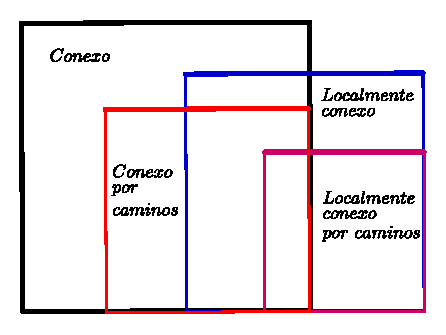
\includegraphics[scale = 1]{img/Comparacion_conexion}
	\caption{Ilustración de las relaciones entre las diferentes nociones de conexión.}
\end{figure}
Veamos un ejemplo de cada, asegurándonos de que hemos hecho bien el dibujo.
\begin{exa}[Ejemplos y contraejemplos]\
	\begin{enumerate}
		\item En la proposición \ref{cam_prop_condSuf} demostramos que un conjunto conexo y localmente conexo por caminos debe ser conexo por caminos, con lo que el dibujo es un fiel reflejo de la realidad, al menos en ese punto.
		\item A la hora de encontrar un espacio conexo por caminos y no localmente conexo nos bastará con coger el conjunto del ejemplo \ref{conex_exa_poliLocal}.
		\item Si al conjunto del ejemplo  \ref{conex_exa_poliLocal} le quitamos el punto $(0,0)$ obtenemos un conjunto conexo, no conexo por caminos que no es localmente conexo.\qedhere
	\end{enumerate}
\end{exa}
Encontrar los contraejemplos restantes requiere un poco más de valor, sangre, sudor, y, por supuesto, muchas lágrimas.
\begin{exa}[Conexo, localmente conexo y no conexo por caminos]
	La recta real con la topología de los complementarios numerables $(\R,\T_{\text{CN}})$ es claramente conexa, ya que dos abiertos cualesquiera se cortan, en efecto, si dos abiertos no triviales $U\cap V=\emptyset$ entonces, tomando complementarios tendríamos que $\R$ es numerable, lo cual es absurdo.
	
	Además, todo abierto $U$ es conexo, esto se debe a que los abiertos relativos de un abierto son los abiertos del espacio ambiente contenidos en $U$. De aquí se deduce que $(\R,\T_{\text{CN}})$ es localmente conexo, ya que basta tomar como base de entornos conexos de un punto $x$ a todos los abiertos que contienen a $x$.
	
	Para ver que no es conexo por caminos usaremos una forma de discurrir muy útil. Supongamos que hay una aplicación $\sigma:[0,1]\to\R$ que conecta dos puntos, digamos $x$ e $y$, y veamos qué debe cumplir para ser un camino.
	
	Si $\sigma$ fuera un camino, entonces $K:=\sigma([0,1])$ sería compacto y conexo. Si $K$ fuera infinito, tendría un subconjunto $F$ numerable, y por tanto cerrado, luego compacto, por ser un cerrado en un compacto. Sin embargo, la topología relativa de $F$ es la discreta por ser un conjunto numerable, lo cual entra en contradicción con su compacidad.
	
	Esto solo nos deja la salida de que $K$ sea finito, y por tanto, $K$ tiene inducida la topología discreta. Como $K$ debe ser también conexo, $K$ tendrá que ser unipuntual. Esto quiere decir que los caminos de $(\R,\T_{\text{CN}})$ únicamente pueden contener a un punto en su traza. Dicho de otra manera, $(\R,\T_{\text{CN}})$ es totalmente disconexo por caminos.
\end{exa}
Únicamente nos queda por encontrar un espacio conexo por caminos, localmente conexo, pero no localmente conexo por caminos. Para ello, de nuevo debemos dibujar un pentagrama en el suelo y rezar $n$ salmos en arameo antiguo.
\begin{exa}[Productos y cocientes de Satán]
	Veamos que el espacio $\X$, definido como sigue, cumple lo que queremos. \[\X:=\frac{[0,1]\times \R}{\{1\}\times \R}\] donde $[0,1]$ tiene la topología usual y $\R$ viene equipado con la topología de los complementarios numerables. La relación de equivalencia que induce este cociente no es más que la que hace corresponder a cada punto consigo mismo e identifica a todos los puntos del segmento $\{1\}\times\R$.
	
	Como los dos factores del producto son localmente conexos, el producto también lo será, así como su cociente. Luego $\X$ es localmente conexo.
	
	$\X$ es conexo por caminos, esto lo deducimos del teorema del pivote. Es claro que cada segmento $y=a$ con $a\in\R$ es un subespacio de $\X$ homeomorfo a $[0,1]$, luego un camino (¡compruébese!). Por tanto, los segmentos $y=a$ son conexos por caminos.
	
	Como la familia de todos estos segmentos cortan a $\{1\}\times \R$, que es un punto de $\X$, hemos encontrado una familia de conexos por caminos de intersección no vacía, que además, cubre el espacio. Esto, por el teorema del pivote quiere decir que $\X$ es conexos por caminos.
	
	Ahora veamos que $\X$ no es localmente conexo por caminos, para ello, tenemos una maravillosa caracterización que nos dice que si lo fuera, entonces los abiertos serían localmente conexos por caminos (ver el lema \ref{cam_lem_caracter} y reflexionar sobre él).
	
	Nuestra tarea pues es encontrar un abierto que no sea localmente conexo por caminos, con un poco de magia encontramos que $A:=\X\setminus (\{1\}\times \R)=[0,1)\times\R$ es un abierto de $\X$ por ser la proyección de un abierto saturado.
	
	$A$ no es localmente conexo por caminos, ya que, al considerar la proyección $p_1$, que es una identificación (por ser sobreyectiva y abierta), luego transforma conserva la local--conexión por caminos, tendríamos que $p_1(A)=\R$. De aquí se desprende que $\R$ con la topología de los complementarios numerables sería localmente conexo por caminos, lo cual es falso.
	
	En efecto, las únicas componentes conexas por caminos de $\R$ son los puntos, que son cerrados, entrando en contradicción con el lema \ref{cam_lem_caracter}.
\end{exa}
Dicho esto, nuestro viaje por la topología general ha concluido. Pero aun debemos cruzar una última frontera, adentrándonos en las entrañas del abstruso, pero a la vez maravilloso mundo de la topología algebraica.